\documentclass[letterpaper]{article}
\usepackage{aaai}
\usepackage{times}
\usepackage{helvet}
\usepackage{courier}
\usepackage{booktabs}
\usepackage{microtype}
\usepackage{amsmath}
\usepackage{amssymb}
\usepackage{graphicx}
\usepackage{float}
\usepackage{hyperref}
\hypersetup{colorlinks=true,linkcolor=[rgb]{0.10,0.20,0.75},citecolor=[rgb]{0.10,0.20,0.75},urlcolor=[rgb]{0.05,0.35,0.85}}
\frenchspacing
\setlength{\pdfpagewidth}{8.5in}
\setlength{\pdfpageheight}{11in}
\pdfinfo{
/Title (Supplementary Material: bioMoR)
/Author (Anonymous Submission)
}
\setcounter{secnumdepth}{1}

\title{Supplementary Material\\
bioMoR: Biology-Guided Mixture-of-Recursions for Efficient and Interpretable Genomic Learning}
\author{Anonymous Submission}

\begin{document}
\maketitle
\appendix

\noindent This supplement collects the additional tables and derivations referenced in the
main paper. Unless stated otherwise, the auxiliary empirical tables here use a $3$-seed
held-out protocol; the $5$-fold cross-validation results reported in the main paper are the
authoritative numbers, and we include these analyses for completeness and transparency.

\section{Baron Training-Cost Curves}
\label{app:curves}
\begin{figure}[h]
\centering
\IfFileExists{figs/baron_loss.pdf}{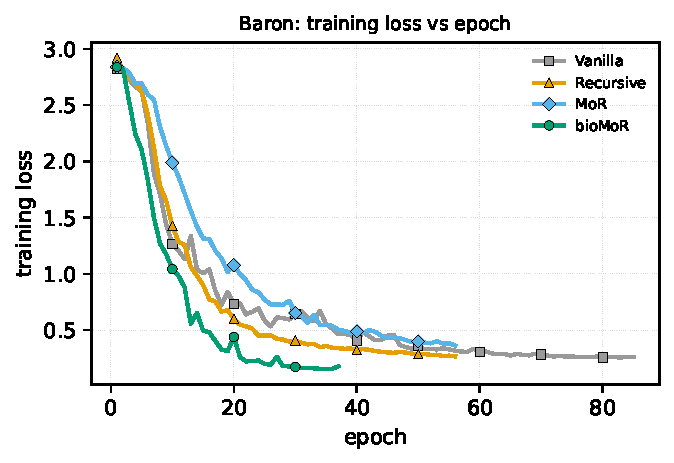
\includegraphics[width=0.49\columnwidth]{figs/baron_loss.pdf}}{}\hfill
\IfFileExists{figs/baron_val_f1.pdf}{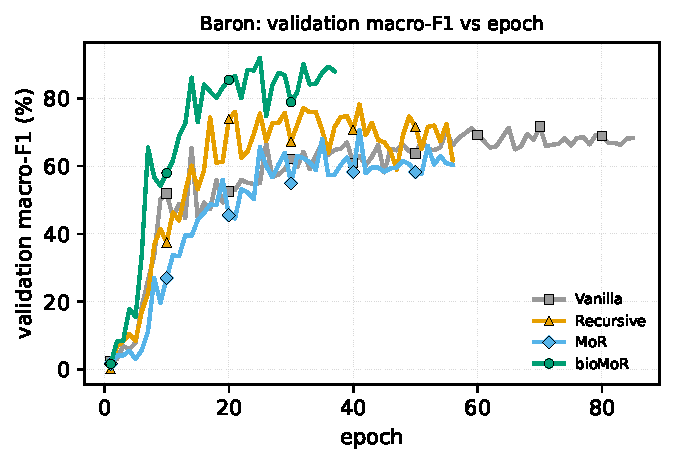
\includegraphics[width=0.49\columnwidth]{figs/baron_val_f1.pdf}}{}%
\caption{\textbf{Full training-cost curves on Baron (pancreas; 5-fold CV).} Training loss (left) and
validation macro-F1 (right) vs.\ measured A100 GPU cost, for all four architectures; lines are the
mean over the same 5 folds as the main table, shaded bands $\pm1$ SD. bioMoR reaches its accuracy
plateau at lower cumulative training cost than the vanilla transformer. The main paper summarises
these curves as an accuracy-vs-cost point diagram (best-loss and best-accuracy operating points).}
\label{fig:baron_curves_full}
\end{figure}

\section{PATH-Comparable Positive-Class F1}
\label{app:posf1}
% Moved from the main paper: the new main-paper Table 3 is the injection-site ablation
% (tab:injection); this positive-class F1 table is a supplementary metric view.
\begin{table}[t]
\centering
\IfFileExists{cv5_posf1_table.tex}{\input{cv5_posf1_table.tex}}{\emph{(positive-class F1 table renders here as runs land)}}
\caption{\textbf{PATH-comparable positive-class F1 on the multi-omics cohorts.} Each
cell is the threshold-calibrated positive-class (progression: metastatic / late-stage)
F1, mean\,$\pm$\,SD over the folds (\%), for the full efficiency ladder --- the
positive-class counterpart of the macro-F1 main-results table (Table~2 of the main paper). Following the
PATH protocol, the operating threshold is tuned on validation to maximise positive-class
F1 and applied to the held-out test fold, with AUROC-based model selection; all other
settings match the main-results table. PM, PC and 3M are the pan-cancer cohorts under mutation$+$CNV, expression, and
tri-modal (all three) inputs; Bladder/Stomach are the BLCA/STAD Reactome cancers.}
\label{tab:posf1}
\end{table}

\section{Model-Size Scaling}
\label{app:scaling}
\begin{table}[t]
\centering
\IfFileExists{cv5_scaling_table.tex}{\resizebox{\columnwidth}{!}{%
\begin{tabular}{c ccc ccc}
\toprule
 & \multicolumn{3}{c}{Single-cell} & \multicolumn{3}{c}{Multi-omics (P-NET)} \\
\cmidrule(lr){2-4}\cmidrule(lr){5-7}
$d_{\text{model}}$ & Vanilla & MoR-gen. & bioMoR & Vanilla & MoR-gen. & bioMoR \\
\midrule
96 & 63.6{\scriptsize$\pm$5.9} & 63.4{\scriptsize$\pm$4.1} & \emph{\scriptsize run\ldots} & \emph{\scriptsize run\ldots} & \emph{\scriptsize run\ldots} & \emph{\scriptsize run\ldots} \\
136 & 65.1{\scriptsize$\pm$5.0} & 64.5{\scriptsize$\pm$5.9} & \emph{\scriptsize run\ldots} & \emph{\scriptsize run\ldots} & \emph{\scriptsize run\ldots} & \emph{\scriptsize run\ldots} \\
192 & 61.8{\scriptsize$\pm$5.1} & 69.7{\scriptsize$\pm$3.3} & \emph{\scriptsize run\ldots} & \emph{\scriptsize run\ldots} & \emph{\scriptsize run\ldots} & \emph{\scriptsize run\ldots} \\
272 & 60.7{\scriptsize$\pm$5.8} & \emph{\scriptsize run\ldots} & \emph{\scriptsize run\ldots} & \emph{\scriptsize run\ldots} & \emph{\scriptsize run\ldots} & \emph{\scriptsize run\ldots} \\
352 & 63.7{\scriptsize$\pm$6.0} & \emph{\scriptsize run\ldots} & \emph{\scriptsize run\ldots} & \emph{\scriptsize run\ldots} & \emph{\scriptsize run\ldots} & \emph{\scriptsize run\ldots} \\
\bottomrule
\end{tabular}}
}{\emph{(scaling table renders here as runs land)}}
\caption{\textbf{Model-size scaling.} Macro-F1 (mean$\pm$SD) across a width sweep
($d_{\mathrm{model}}\in\{96,\dots,352\}$) for Vanilla, MoR-general and bioMoR, averaged over
the $8$ single-cell and $3$ Reactome multi-omics suites. bioMoR holds a flat, high accuracy across widths
while the vanilla stack---at $4\times$ the recursion-stack parameters---degrades.}
\label{fig:scaling_cv5}
\end{table}

\begin{table}[t]
\centering
\resizebox{\columnwidth}{!}{%
\begin{tabular}{lcccccc}
\toprule
Dataset & $M{=}128$ & $M{=}256$ & $M{=}512$ & $M{=}1024$ & $M{=}2048$ & Linear (all feat.) \\
\midrule
Baron & 79.1\,$\pm$\,2.8 & 78.1\,$\pm$\,1.4 & 79.6\,$\pm$\,4.4 & 82.6\,$\pm$\,2.0 & 80.4\,$\pm$\,2.1 & 91.1\,$\pm$\,2.0 \\
Lung & 79.1\,$\pm$\,1.2 & 80.2\,$\pm$\,0.8 & 79.8\,$\pm$\,1.9 & 81.3\,$\pm$\,2.0 & 81.1\,$\pm$\,1.9 & 74.8\,$\pm$\,0.2 \\
Muraro & 75.3\,$\pm$\,6.4 & 72.4\,$\pm$\,2.7 & 68.3\,$\pm$\,3.3 & 75.7\,$\pm$\,4.5 & 73.8\,$\pm$\,6.0 & 95.7\,$\pm$\,2.2 \\
Oesophagus & 69.6\,$\pm$\,1.4 & 69.8\,$\pm$\,0.6 & 71.5\,$\pm$\,1.6 & 73.6\,$\pm$\,0.5 & 72.2\,$\pm$\,1.6 & 69.5\,$\pm$\,1.1 \\
Segerstolpe & 71.4\,$\pm$\,5.3 & 70.3\,$\pm$\,4.1 & 73.8\,$\pm$\,5.4 & 69.4\,$\pm$\,14.7 & 68.3\,$\pm$\,3.3 & 89.5\,$\pm$\,5.0 \\
Spleen & 58.2\,$\pm$\,0.9 & 58.6\,$\pm$\,1.6 & 59.9\,$\pm$\,0.8 & 61.1\,$\pm$\,2.3 & 61.6\,$\pm$\,4.0 & 64.7\,$\pm$\,0.1 \\
T-cell & 68.9\,$\pm$\,1.0 & 69.9\,$\pm$\,0.3 & 71.5\,$\pm$\,0.4 & 71.8\,$\pm$\,2.3 & 73.0\,$\pm$\,0.3 & 78.1\,$\pm$\,0.3 \\
Xin & 64.7\,$\pm$\,9.4 & 64.8\,$\pm$\,6.0 & 63.7\,$\pm$\,10.3 & 64.1\,$\pm$\,0.6 & 62.1\,$\pm$\,2.8 & 97.4\,$\pm$\,0.6 \\
\midrule
\textbf{Mean macro-F1} & \textbf{70.8} & \textbf{70.5} & \textbf{71.0} & \textbf{72.5} & \textbf{71.6} & \textbf{82.6} \\
\bottomrule
\end{tabular}}
\caption{\textbf{Marker-budget headroom (3-seed held-out).} Single-cell macro-F1 as the
marker budget $M$ grows, against the full-feature linear baseline. Even when every feature
is a marker, a residual to the linear model remains, so the gap is architectural rather than
a token-budget limitation.}
\label{tab:mbudget}
\end{table}

\begin{table}[t]
\centering
\resizebox{\columnwidth}{!}{%
\begin{tabular}{lcccc}
\toprule
Dataset & Learned (random init) & $+$ bio warm-start & $+$ stronger init & $+$ annealed anchor \\
\midrule
Baron & 82.3\,$\pm$\,2.2 & 80.9\,$\pm$\,3.8 & 81.6\,$\pm$\,1.8 & 66.8\,$\pm$\,6.2 \\
Lung & 79.5\,$\pm$\,1.4 & 79.8\,$\pm$\,0.8 & 78.4\,$\pm$\,0.6 & 70.0\,$\pm$\,2.7 \\
Muraro & 74.5\,$\pm$\,5.4 & 75.3\,$\pm$\,4.9 & 76.6\,$\pm$\,5.4 & 75.9\,$\pm$\,9.3 \\
Oesophagus & 69.3\,$\pm$\,0.7 & 71.1\,$\pm$\,0.9 & 70.2\,$\pm$\,1.0 & 57.4\,$\pm$\,2.6 \\
Segerstolpe & 74.0\,$\pm$\,5.3 & 69.9\,$\pm$\,7.4 & 74.5\,$\pm$\,5.7 & 53.0\,$\pm$\,5.0 \\
Spleen & 59.0\,$\pm$\,0.2 & 59.1\,$\pm$\,0.7 & 58.7\,$\pm$\,1.2 & 52.5\,$\pm$\,1.2 \\
T-cell & 68.9\,$\pm$\,0.7 & 69.1\,$\pm$\,1.1 & 69.0\,$\pm$\,0.6 & 54.7\,$\pm$\,2.4 \\
Xin & 69.2\,$\pm$\,5.0 & 67.2\,$\pm$\,8.4 & 68.5\,$\pm$\,6.1 & 69.5\,$\pm$\,7.7 \\
\midrule
\textbf{Mean macro-F1} & \textbf{72.1} & \textbf{71.5} & \textbf{72.2} & \textbf{62.5} \\
\quad $\Delta$ vs.\ random & $+0.0$ & $-0.6$ & $+0.1$ & $-9.6$ \\
\bottomrule
\end{tabular}}
\caption{\textbf{Stress-testing the biological warm-start} (single-cell macro-F1,
mean$\pm$std). From a randomly-initialised learned graph we add a biological warm-start,
then a stronger init, then an annealed anchor $\lambda(t)\lVert A_{\text{learned}}-A_{\text{bio}}\rVert_F^2$
that keeps the graph near biology early. The $\Delta$ row is the mean gain over random
init; forcing biology in more strongly does not beat learning the graph from data.}
\label{tab:anchor}
\end{table}

\begin{table}[t]
\centering
\resizebox{\columnwidth}{!}{%
\begin{tabular}{lccc}
\toprule
Cohort & bioMoR (mut+CNV) & Geneformer & scGPT \\
\midrule
Prostate & 78.2\,$\pm$\,2.2 & 78.2\,$\pm$\,3.3 & 40.1\,$\pm$\,0.0 \\
BLCA (bladder) & 40.9\,$\pm$\,1.9 & 47.7\,$\pm$\,3.7 & 40.4\,$\pm$\,0.0 \\
STAD (stomach) & 52.2\,$\pm$\,6.8 & 46.1\,$\pm$\,5.5 & 35.7\,$\pm$\,0.0 \\
\midrule
\textbf{Mean} & \textbf{57.1} & \textbf{57.3} & \textbf{38.7} \\
\bottomrule
\end{tabular}}
\caption{\textbf{bioMoR vs.\ gene-vocabulary foundation models} on the Reactome multi-omics cohorts
(macro-F1, mean$\pm$std over seeds). Geneformer (fine-tuned) and scGPT (frozen embedding
$+$ logistic probe) are mapped onto each cohort's HUGO gene symbols with a per-gene
mutation/copy-number alteration burden, on the same splits as bioMoR. Bulk DNA-alteration
input is out-of-distribution for these single-cell-RNA models.}
\label{tab:fm}
\end{table}

% Calibration / uncertainty table removed.

\begin{table}[t]
\centering
\resizebox{0.85\columnwidth}{!}{%
\begin{tabular}{lccc}
\toprule
Depth $K$ & Shared (ours) & Independent & Reduction \\
\midrule
1 & 74{,}880 & 74{,}880 & 1$\times$ \\
2 & 74{,}880 & 149{,}760 & 2$\times$ \\
3 & 74{,}880 & 224{,}640 & 3$\times$ \\
4 & 74{,}880 & 299{,}520 & 4$\times$ \\
6 & 74{,}880 & 449{,}280 & 6$\times$ \\
8 & 74{,}880 & 599{,}040 & 8$\times$ \\
\bottomrule
\end{tabular}}
\caption{\textbf{Parameter reduction.} One shared block versus $K$ independent layers at
matched width: an exact $K\times$ reduction, present before any training.}
\label{tab:param}
\end{table}

\begin{table}[t]
\centering
\resizebox{\columnwidth}{!}{%
\begin{tabular}{lccccc}
\toprule
Dataset & $M{=}16$ & $M{=}32$ & $M{=}64$ & $M{=}128$ & $M{=}256$ \\
\midrule
\multicolumn{6}{l}{\emph{Single-cell (genomap)}} \\
\quad Baron & 33.7\,$\pm$\,7.1 & 38.5\,$\pm$\,2.1 & 53.9\,$\pm$\,1.9 & 62.6\,$\pm$\,5.1 & 66.9\,$\pm$\,3.4 \\
\quad Lung & 30.8\,$\pm$\,5.9 & 38.1\,$\pm$\,1.7 & 61.5\,$\pm$\,1.9 & 71.4\,$\pm$\,1.1 & 78.4\,$\pm$\,0.8 \\
\quad Muraro & 55.8\,$\pm$\,3.6 & 59.4\,$\pm$\,1.3 & 67.9\,$\pm$\,5.6 & 68.5\,$\pm$\,4.1 & 76.2\,$\pm$\,5.2 \\
\quad Oeso. & 23.1\,$\pm$\,1.3 & 30.2\,$\pm$\,3.9 & 42.0\,$\pm$\,2.4 & 53.9\,$\pm$\,4.4 & 63.2\,$\pm$\,2.4 \\
\quad Seger. & 41.2\,$\pm$\,12.1 & 45.3\,$\pm$\,5.6 & 59.3\,$\pm$\,4.0 & 59.1\,$\pm$\,1.6 & 55.4\,$\pm$\,7.0 \\
\quad Spleen & 18.7\,$\pm$\,2.4 & 26.8\,$\pm$\,3.0 & 38.1\,$\pm$\,2.3 & 48.1\,$\pm$\,5.0 & 59.4\,$\pm$\,0.9 \\
\quad T-cell & 25.5\,$\pm$\,3.2 & 36.6\,$\pm$\,5.4 & 43.1\,$\pm$\,5.2 & 47.4\,$\pm$\,2.2 & 61.5\,$\pm$\,1.7 \\
\quad Xin & 50.5\,$\pm$\,5.9 & 46.2\,$\pm$\,1.6 & 60.8\,$\pm$\,5.6 & 64.1\,$\pm$\,3.3 & 72.4\,$\pm$\,11.7 \\
\midrule
\multicolumn{6}{l}{\emph{Multi-omics (Reactome)}} \\
\quad Prostate & 74.3\,$\pm$\,3.0 & 74.7\,$\pm$\,2.7 & 78.0\,$\pm$\,3.0 & 76.7\,$\pm$\,2.6 & 77.3\,$\pm$\,0.2 \\
\quad BLCA (bladder) & 49.8\,$\pm$\,2.2 & 46.0\,$\pm$\,3.1 & 49.3\,$\pm$\,2.5 & 48.1\,$\pm$\,6.8 & 55.7\,$\pm$\,3.5 \\
\quad STAD (stomach) & 54.2\,$\pm$\,3.1 & 51.0\,$\pm$\,2.2 & 44.0\,$\pm$\,5.6 & 51.2\,$\pm$\,2.8 & 49.4\,$\pm$\,4.1 \\
\midrule
\textbf{Mean macro-F1} & \textbf{41.6} & \textbf{44.8} & \textbf{54.4} & \textbf{59.2} & \textbf{65.1} \\
\bottomrule
\end{tabular}}
\caption{\textbf{Marker-token budget.} Macro-F1 (mean$\pm$std over 3 seeds) as
the marker budget $M$ shrinks from 256 to 16. A few dozen to a few hundred tokens recover
most of the full-gene accuracy. Bottom row: mean over the $11$ single-cell and Reactome multi-omics
datasets included in this sweep (the pan-cancer settings are omitted here).}
\label{tab:token}
\end{table}



\section{Dataset Details}
\label{app:data}
We use $14$ datasets: $8$ genomap single-cell datasets \cite{islam2023cartography}, each an
expression matrix with cell-type labels and a fixed stratified split -- Baron, Lung, Muraro, Oesophagus,
Segerstolpe, Spleen, T-cell and Xin -- $3$ Reactome multi-omics
cohorts --- prostate, bladder (BLCA), stomach (STAD) cancer --- whose fixed Reactome pathway tokens pool mutation,
copy-number and expression channels, and $3$ pan-cancer TCGA settings of a binary
primary-vs-metastatic task (PM, mutation$+$CNV; PC, expression; 3M, tri-modal). Per-dataset
sample, feature and class counts are read directly from the result files and summarised in
Table~\ref{tab:datasets}.

\begin{table}[h]
\centering
\resizebox{\columnwidth}{!}{%
\begin{tabular}{llrrr}
\toprule
Dataset & Modality & Samples & Features & Classes \\
\midrule
Baron & single-cell & 8{,}569 & 2{,}000 & 13 \\
Lung & single-cell & 57{,}020 & 1{,}089 & 25 \\
Muraro & single-cell & 2{,}122 & 2{,}000 & 9 \\
Oesophagus & single-cell & 87{,}947 & 1{,}089 & 18 \\
Segerstolpe & single-cell & 2{,}127 & 2{,}000 & 11 \\
Spleen & single-cell & 94{,}129 & 1{,}089 & 28 \\
T-cell & single-cell & 24{,}007 & 1{,}089 & 7 \\
Xin & single-cell & 1{,}492 & 2{,}000 & 4 \\
\midrule
Prostate & multi-omics & 1{,}011 & 1{,}223 & 2 \\
BLCA (bladder) & multi-omics & 404 & 1{,}258 & 2 \\
STAD (stomach) & multi-omics & 414 & 1{,}258 & 2 \\
Pan-cancer PM (mut$+$CNV) & multi-omics & 8{,}893 & 10{,}333 & 2 \\
Pan-cancer PC (expression) & multi-omics & 8{,}586 & 10{,}013 & 2 \\
Pan-cancer 3M (tri-modal) & multi-omics & 8{,}586 & 9{,}880 & 2 \\
\bottomrule
\end{tabular}}
\caption{The datasets used throughout ($14$ in total): $8$ genomap single-cell suites,
$3$ Reactome multi-omics cohorts, and $3$ pan-cancer TCGA settings (PM, PC, 3M).
Counts are read directly from the result files.}
\label{tab:datasets}
\end{table}

\section{Implementation Details and Hyperparameters}
\label{app:hparams}
All settings below are held \emph{fixed across every dataset and every variant} (no per-dataset
tuning); the only quantities we vary are those explicitly swept in a reported study (marker/token
budget $M$ in the scaling table, recursion depth $K$ in the ladder). This keeps every comparison in
the main results paired.

\paragraph{Optimisation and protocol.}
We train with AdamW (learning rate $3\times10^{-4}$, weight decay $10^{-2}$), dropout $0.1$, for up
to $100$ epochs with early stopping on validation macro-F1 (patience $15$). The protocol is
$5$-fold stratified cross-validation (seed $42$; $20\%$ test, $10\%$-of-train validation), with
per-gene $z$-scoring fit on the training fold only. Single-cell models use $d_{\mathrm{model}}{=}96$
and $M{=}128$ learnable marker tokens; multi-omics models use $d_{\mathrm{model}}{=}128$, $M{=}256$
fixed Reactome pathway tokens, and batch size $32$. The weight-shared block is applied up to
$K{=}4$ times by default.

\paragraph{Router budgets.}
Expert-choice routing uses a fixed \emph{capacity funnel}: at recursion step $t$ the router keeps a
fraction $c_t=\max(0.75,\,1-0.25\,t)$ of the tokens, i.e.\ $c=(1.00,\,0.75,\,0.75,\,0.75)$ at
$K{=}4$ (all tokens pass step~$0$, then a $0.75$ floor thereafter; the floor is exposed as
\texttt{RMT\_CAP\_FLOOR}). The floor is deliberately gentle---because the classifier mean-pools the
$M$ marker tokens, freezing too many too early starves the pooled vector, and a $0.5$ floor made
$K{=}4$ the weakest depth. Token-choice routing instead lets each token self-gate a single depth in
$\{1,\dots,K\}$ (top-$1$ over depths), so its budget is emergent rather than fixed. The router gate
scale ($\alpha{=}1.0$) and temperature ($\tau{=}1.0$) are left at their neutral defaults.

\paragraph{Balancing coefficients.}
Expert-choice is load-balanced by construction (the funnel fixes per-step capacity), so it carries
no balancing loss. Token-choice adds a Switch-style load-balancing term
\cite{shazeer2017outrageously} over the $K$ depths with weight $0.1$, plus a router $z$-loss
(logit-magnitude regulariser) with weight $10^{-3}$. When the biological prior is injected at the
router it enters as an additive centrality bias on the depth logits with initial strength
$\beta_0{=}1.0$, annealed toward $0$ over training; the learned interaction graph is mixed into the
token embeddings through a sigmoid-bounded, \emph{learnable} coefficient initialised at $\lambda{=}0.3$.
A marker-sufficiency auxiliary head (weight $1.0$) probes the pre-recursion marker panel; the total
objective is the classification cross-entropy plus these auxiliary and balancing terms.

\section{Effective-FLOPs Accounting}
\label{app:flops}
The compute numbers report per-sample FLOPs of the recursive transformer stack, the
only component routing changes. One application of the shared block to $a$ tokens costs
$\phi(a)=4a^2 d + 4\,a\,d\,d_{\mathrm{ff}}$; the nominal fixed-depth cost is
$\Phi_{\mathrm{nom}}=K\,\phi(M)$ and the effective cost sums one block over the tokens
active at each step, $\Phi_{\mathrm{eff}}=\sum_{t=1}^{K}\phi(a_t)$, where $a_t$ is the
mean number of markers the expert-choice funnel keeps at step $t$. Gene embedding and
marker selection are $\mathcal{O}(Nd)$, identical across routing modes, and excluded
from this stack-level comparison.

\paragraph{End-to-end accounting.}
For completeness we account for the whole forward pass, not only the stack. Three parts
scale with the full gene count $N$: gene embedding $\Theta(Nd)$; the cross-attention
marker router, whose $M$ queries attend over all $N$ gene keys at
$\Theta(MNd)$; and the optional gene-graph smoother, which at rank $r$ costs
$\Theta(Nr)$ (never the $N^2$ dense form). Everything after marker selection -- the
recursive stack, pooling and head -- scales with the compressed budget $M\ll N$ at
$\Theta(M^2d)$ per pass. So the router's $\Theta(MNd)$ term dominates the $N$-scaling
and is \emph{linear} in $N$ (versus the $\Theta(N^2 d)$ self-attention a full-gene
transformer would pay), while the quadratic cost is paid only on the $M$ markers. The
architecture ablations of the main-paper efficiency ladder vary only the stack, so the stack-level
ratios there are the correct comparison for the routing/sharing claims; the router and
embedding terms are shared by every variant. Measured wall-clock and peak-memory
profiling on matched hardware is a straightforward addition we leave to the camera-ready.

\section{Theoretical Foundation of the Router}
\label{app:theory}
This appendix gives the mathematical and biological grounding for bioMoR's
biology-informed router.

\paragraph{Routing as conditional computation.}
The router implements \emph{conditional computation}: a learned policy routes each token
to a token-specific amount of compute, the gating principle of sparsely-gated mixtures
of experts \cite{shazeer2017outrageously}, reused by Mixture-of-Depths
\cite{raposo2024mixture} and Mixture-of-Recursions \cite{bae2025mixture}; the
``experts'' here are recursion \emph{depths} of one shared block, which couples adaptive
computation \cite{graves2016adaptive} to weight sharing.

\paragraph{The differentiable handle.}
The discrete top-$k$ has zero gradient almost everywhere, so bioMoR keeps the soft
probability of the chosen route as a multiplicative \emph{gate} on the block output,
$\mathbf{o}_m=g_m\,f_\theta(\mathbf{h}_m)$ with $g_m=\sigma(\tilde r_m)$. Because $g_m$
is smooth in $\mathbf{w}_r$, the chain
$\mathcal{L}\!\leftarrow\!\mathbf{o}_m\!\leftarrow\!g_m\!\leftarrow\!\mathbf{w}_r$ is
unbroken: the hard choice routes, the soft gate carries the gradient. The biological
prior of the routing logit of the main paper (Eq.~1) is an additive constant in this logit, so it shifts
the decision without breaking this path.

\paragraph{Biological foundation of the prior.}
Two facts from single-cell biology motivate the prior. A small set of \emph{marker}
genes carries most discriminative signal
\cite{ianevski2022fully,franzen2019panglaodb,hu2023cellmarker}, so compute should be
allocated unevenly. And gene co-expression networks are approximately scale-free: a few
high-degree \emph{hub} genes (master regulators) exert outsized influence. We
operationalise ``hub'' as eigenvector centrality on the genomap co-expression graph
$\mathbf{W}$: the leading eigenvector $\mathbf{v}$ of
$\mathbf{W}\mathbf{v}=\lambda\mathbf{v}$ scores each gene by the centrality of its
neighbours, recursively, and we $z$-score it to form $\pi$.

\paragraph{Empirical-Bayes reading.}
The routing logit of the main paper (Eq.~1) is a log-linear prior on the routing decision, with
$\beta_t\,\pi_m$ a Gaussian-like prior mean and $\beta_t=\beta_0(1-\text{progress})$ a
shrinkage strength that decays as data evidence accumulates: prior-dominated when the
likelihood is uninformative (early training), data-dominated later.

\paragraph{Leakage safety.}
$\mathbf{W}$ is computed from training-split \emph{expression only}; no cell-type label
enters it. The prior therefore injects network topology, not the answer, which is why a
gene-discovery claim under this prior is not circular, unlike a prior built from curated
cell-type marker lists.

\paragraph{Optional pathway-graph smoothing.}
The additive bias treats genes independently. Co-pathway genes should route coherently,
which one obtains by smoothing the logits over $\mathbf{W}$ with the normalised
Laplacian $\mathbf{L}=\mathbf{I}-\mathbf{D}^{-1/2}\mathbf{W}\mathbf{D}^{-1/2}$,
$\hat{\mathbf{r}}^{(t)}=\tilde{\mathbf{r}}^{(t)}-\gamma\,\mathbf{L}\tilde{\mathbf{r}}^{(t)}$
(graph-Laplacian regularisation): a gene borrows routing strength from its network
neighbours. This is one sparse matrix-vector product per step and adds no transformer
parameters; we expose it as an option and leave its evaluation to future work.

\section{Routing-Depth Visualisation}
\label{app:depth}
\begin{figure}[h]
\centering
\IfFileExists{figs/fig2_depth.pdf}{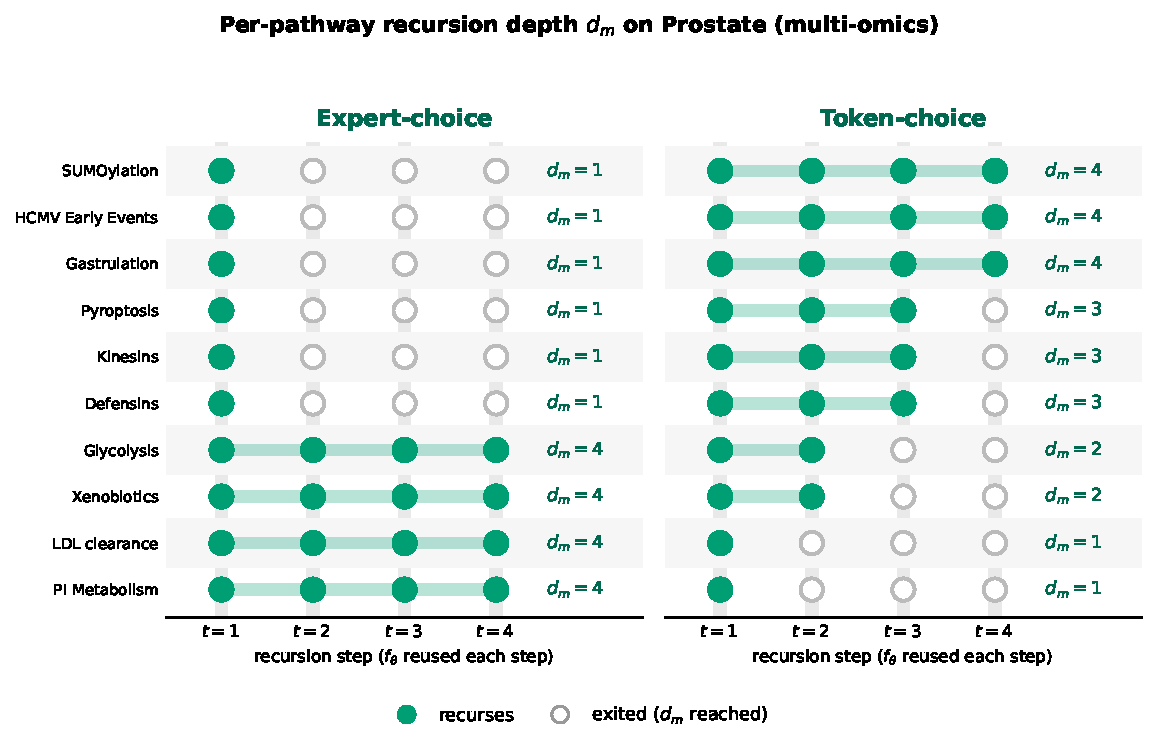
\includegraphics[width=\columnwidth]{figs/fig2_depth.pdf}}{}%
\caption{\textbf{Two routing modes assign per-pathway depth $d_m$} (real Prostate tokens;
$\bullet$ recurses, $\circ$ exited; the block $f_\theta$ is reused up to $K{=}4$, so depth adds
no parameters). Expert-choice fixes capacity per step; token-choice lets each pathway self-gate
its depth.}
\label{fig:mor_supp}
\end{figure}

\IfFileExists{pm_depth_tables.tex}{\input{pm_depth_tables.tex}}{\emph{(per-pathway PM depth tables render here once scripts/build\_pm\_depth\_tables.py runs)}}

\section{Proofs for the Theoretical Analysis}
\label{app:proofs}
We use the signal-plus-noise model of the main text: $x=z+\varepsilon$,
$\varepsilon\sim(0,\sigma^2 I_G)$, $\varepsilon\perp z$, $\mathbb{E}z=0$,
$\Sigma=\mathbb{E}[zz^\top]=\sum_k s_k u_k u_k^\top$ with $s_1\ge s_2\ge\cdots\ge0$ and
orthonormal $\{u_k\}$; at least one $s_k>0$. The propagation is the linear filter
$T_\lambda=(1-\lambda)I+\lambda A$, $A=\tilde E\tilde E^\top\succeq0$, $\mathrm{rank}(A)\le r$,
and $R(T)=\mathbb{E}\lVert Tx-z\rVert^2$. Regimes: $B_0$ ($T{=}I$) $\subseteq B_1$ ($A{=}0$)
$\subseteq B_2$ (learned $A$).

\paragraph{Lemma~1 (Spectral decoupling).} For symmetric $T=\sum_k f_k u_ku_k^\top$,
$R(T)=\sum_k[(1-f_k)^2 s_k+f_k^2\sigma^2]$.
\emph{Proof.} $R(T)=\mathbb{E}\lVert(T-I)z\rVert^2+\mathbb{E}\lVert T\varepsilon\rVert^2$ (cross term
vanishes as $\varepsilon\perp z$). By trace cyclicity the first is
$\mathrm{tr}((T-I)\Sigma(T-I)^\top)=\sum_k(f_k-1)^2 s_k$ and the second is
$\sigma^2\mathrm{tr}(TT^\top)=\sigma^2\sum_k f_k^2$. $\square$

\paragraph{Lemma~2 (Per-direction Wiener optimum).} Each summand is strictly convex in $f_k$ and
minimised at $f_k^\star=s_k/(s_k+\sigma^2)\in[0,1)$ with residual $s_k\sigma^2/(s_k+\sigma^2)$.
\emph{Proof.} $g(f)=(1-f)^2 s_k+f^2\sigma^2$ has $g'(f)=-2(1-f)s_k+2f\sigma^2$, vanishing at
$f_k^\star$; $g''=2(s_k+\sigma^2)>0$. Substituting gives the residual. The signal-preservation
gain over the fully-shrunk value $g(0)=s_k$ is $s_k-\frac{s_k\sigma^2}{s_k+\sigma^2}=\frac{s_k^2}{s_k+\sigma^2}$. $\square$

\paragraph{Lemma~3 (Realizability).} For any $\{f_i\}_{i\le r}\subset[0,1]$ on any orthonormal
$\{v_i\}_{i\le r}$ there exist $\lambda\in[0,1]$ and PSD $A=\tilde E\tilde E^\top$ of rank $\le r$
with $T_\lambda v_i=f_i v_i$. \emph{Proof.} Take $\lambda=1$, $\mu_i=(f_i-(1-\lambda))/\lambda=f_i\ge0$,
$A=\sum_{i\le r}\mu_i v_iv_i^\top$, $\tilde E=[\sqrt{\mu_1}v_1,\dots,\sqrt{\mu_r}v_r]$; on
$\mathrm{span}\{v_i\}^\perp$, $A{=}0$ so $T_\lambda=(1-\lambda)I$ only further shrinks noise
directions. $\square$

\paragraph{Theorem~1.} Monotonicity is immediate from the nesting $B_0\subseteq B_1\subseteq B_2$
(min of the same objective over a larger set). $R^\star(B_0)=G\sigma^2$ ($f_k\equiv1$ in
Lemma~1). By Lemma~3 place $v_i{=}u_i$, $f_i{=}f_i^\star$ for $i\le r$ and $f_k{=}1-\lambda$ on the
tail; Lemma~2 gives, per top-$r$ direction, a saving
$\sigma^2-\frac{s_i\sigma^2}{s_i+\sigma^2}=\frac{\sigma^4}{s_i+\sigma^2}$, equivalently a
signal-preservation gain $\frac{s_i^2}{s_i+\sigma^2}$, and $\lambda\to0$ recovers $\sigma^2$ on the
tail. Hence $R^\star(B_0)-R^\star(B_2)\ge\sum_{i\le r}\frac{s_i^2}{s_i+\sigma^2}>0$. $\square$

\paragraph{Proposition~1 (No graph cannot close the gap).} If $s_i\ne s_j$ for some $i,j\le r$
then $R^\star(B_1)>R^\star(B_2)$. \emph{Proof.} $B_1$ forces one scalar $f_k\equiv f$ (since
$A{=}0$); minimising Lemma~1 over a single $f$ gives $\hat f=\mathrm{tr}\Sigma/(\mathrm{tr}\Sigma+G\sigma^2)$,
whereas the per-direction optima $f_i^\star$ differ when the $s_i$ differ. A convex objective under
the equality constraint ``all $f_k$ equal'' exceeds its unconstrained minimum whenever the latter
violates the constraint. $\square$

\paragraph{Proposition~2 (Task-risk bound).} If the head $\Phi$ is $L_\Phi$-Lipschitz and the label
depends on the clean signal through the selection statistics $Wz$, then
$\mathbb{E}\lVert\Phi(WTx)-\Phi(Wz)\rVert\le L_\Phi\lVert W\rVert_2\sqrt{R(T)}$; minimising $R$ over
$B_2$ strictly tightens this over $B_0$ by Theorem~1. \emph{Proof.} Lipschitzness and the
operator-norm inequality bound the LHS by $L_\Phi\lVert W\rVert_2\lVert Tx-z\rVert$; take
expectations and apply Jensen. $\square$

\paragraph{Theorem~2 (Router monotone-safety).} With router logit
$\ell_t=\rho_\theta^{(t)}(H)+\Phi_t(AH)^\top$ and $A$ row-stochastic, setting $\Phi{=}0$ recovers
the baseline router exactly, so $\Theta_0\subset\Theta_G$ and $R^\star(\Theta_G)\le R^\star(\Theta_0)$;
gradient flow from $\Phi{=}0$ has $\tfrac{d}{d\tau}L=-\lVert\nabla L\rVert^2\le0$, so the trained
router attains loss $\le$ the baseline. Strictness: a baseline router is $\sigma(h_m)$-measurable
and cannot separate two tokens with equal $h_m$ but different neighbourhoods $(AH)_m$, incurring a
fixed excess $\delta>0$ that a suitable $\Phi$ removes. $\square$

\paragraph{Corollary~1 (Both sites best).} The joint family contains embedding-only ($\Phi{=}0$)
and router-only ($\lambda{=}0$) as no-op restrictions, so
$R^\star_{\mathrm{both}}\le\min\{R^\star_{\mathrm{emb}},R^\star_{\mathrm{rt}}\}\le R^\star_{\mathrm{none}}$
by monotonicity of the min over set inclusion. $\square$

\section{Low-Rank Propagation, Over-Smoothing, and Rare Cells}
\label{app:oversmooth}
The denoising filter and the over-smoothing failure mode are two ends of the same spectral dial. Let
$A=\tilde E\tilde E^\top$ have eigendecomposition $A=\sum_k a_k w_kw_k^\top$ with $a_k\ge0$ and
$a_k{=}0$ for $k>r$ (the range of $\tilde E$ is $r$-dimensional). Then $T_\lambda=(1-\lambda)I+\lambda A$
is simultaneously diagonalised, with eigenvalues
\[
\mu_k(\lambda)\;=\;1-\lambda+\lambda a_k ,
\]
so on the $r$ graph directions $T_\lambda$ scales by $1-\lambda+\lambda a_k$ and on the orthogonal
complement it acts as the scalar $1-\lambda$.

\paragraph{Spectral view of over-smoothing.} As $\lambda\to1$ the off-range eigenvalue $1-\lambda\to0$:
every direction outside $\mathrm{span}(\tilde E)$ is annihilated and token features collapse onto the
$r$-dimensional graph subspace, the discrete analogue of graph over-smoothing (repeated propagation
driving representations toward a low-rank fixed point). The \emph{spectral gap} that controls how fast
this happens is $\min_k \mu_k - (1-\lambda) = \lambda\,a_{\min}^{+}$ on the range versus $1-\lambda$
off it; a large $\lambda$ widens the gap and accelerates the collapse. Because bioMoR \emph{learns}
$\lambda$ through a sigmoid (initialised at $0.3$; App.~\ref{app:hparams}) rather than fixing it at the
denoising-maximal value, and because the residual identity path guarantees $\mu_k\ge 1-\lambda>0$ for
all $k$, no direction is fully annihilated: the operator is a \emph{bounded} smoother, not a projector.

\paragraph{Rare-cell implication.} Rare populations are precisely the directions this dial threatens.
Their signal typically lives in low-variance modes ($s_k$ small, and frequently outside the dominant
top-$r$ subspace), where the Wiener-optimal gain $f_k^\star=s_k/(s_k+\sigma^2)$ from Lemma~2 is already
small; additional smoothing ($\mu_k\to$ off-range $1-\lambda$) drives the effective gain toward zero
and erases the very directions that separate a rare type from the bulk. The learned bounded $\lambda$
is therefore not a convenience but the mechanism that protects rare-cell discriminability while still
denoising the high-variance modes ($s_k\gg\sigma^2$, where $f_k^\star\to1$ and smoothing is safe).
A second structural safeguard is that propagation acts on the $M\ll N$ marker/pathway \emph{tokens},
not on cells: it mixes feature channels within a token but cannot average two cells of different type
into one, so it cannot induce the cell-level homogenisation that over-smoothing causes in
cell--cell-graph GNNs.

\paragraph{Prediction and diagnostics.} This analysis predicts a \emph{graded} benefit: the learned
graph should help most where the raw per-feature signal is weak (denoising dominates) and little where
classes are already separable (smoothing is redundant and risks the rare-cell modes) --- exactly the
pattern in the main-results table (largest gains on the hard single-cell suites and the multi-omics
cohorts, negligible where a task is near-saturated). Two direct falsifiers we leave to future work: a
per-class recall breakdown restricted to the rarest populations (over-smoothing predicts the learned
graph should never \emph{lower} rare-class recall relative to no graph, given the bounded $\lambda$),
and a sweep of $\lambda$ against the induced spectral gap $\lambda a_{\min}^{+}$ measuring where the
denoising/over-smoothing trade-off turns.

\bibliographystyle{aaai}
\bibliography{refs}
\end{document}
